%%==================================================
%% chapter01.tex for BIT Master Thesis
%% modified by yang yating
%% version: 0.1
%% last update: Dec 25th, 2016
%%==================================================
\chapter{绪论}
\label{chap:intro}
\section{本论文研究的目的和意义}

在未来战争中,仅靠单架无人机自主作战无法适应复杂多样的战场环境,而具备协同作战的无人机编队能更好地完成任务,与单架无人机相比具有作战效率高、
视野广阔等优势,可实现对目标的全方位立体监视,对地精确攻击。另外,无人机紧密编队可以实现长航任务中无人机的空中加油,对接等任务,如图\ref{fig:c01-meaning-1}。编队飞行作为
无人机研究领域的热点与难点问题,涉及多项关键技术,例如:队形设计、自主编队、队形保持变换、协调通信等。无人机自主编队控制是实现集群作战的关键技
术。

固定翼无人机以紧密编队的形式飞行,如迁徙的鸟儿一样,可以减少整体的飞行阻力并且减少燃料消耗。整体编队产生的效果将会与精心设计的、具有良好的气动
外形的飞行器相媲美。但是,按照相关文献显示,如果固定翼编队的控制精度无法达到要求精度的10\%,那么最优的减租效果可能会被削减30\%。
\begin{figure}
  \centering
  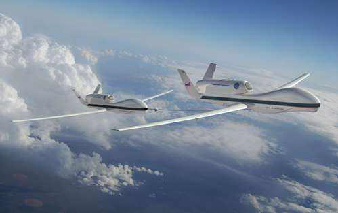
\includegraphics[width=0.75\textwidth]{figures/c01-meaning-1}
  \caption{无人机编队加受油}\label{fig:c01-meaning-1}
 \end{figure}

%\upcite{Takahashi1996Structure,Xia2002Analysis,Jiang1989,Mao2000Motion,Feng1998}%这个是文献引用上标
\section{国内外研究现状及发展趋势}
%\label{sec:***} 可标注label
现如今的无人机自动驾驶仪的结构多为导航模块、位置控制控制模块(外环)以及姿态控制模块(内环);导航模块产生期望位置,位置控制模块由期望位置产生
期望姿态角,姿态控制模块由期望姿态角产生最终的伺服系统的控制量。现如今的低成本无人机所使用的传感器硬件精度比较低,均为消费级别,如果不考虑传感
器的精度问题而设计控制方案,很可能导致整体编队的控制精度下降。现如今已经存在的大部分编队控制算法,未考虑无人机的动力学模型,即只考虑飞机的质点
运动学以及质点动力学条件下提出的导航方法,最终产生的飞行器的控制量为无人机航迹坐标系下的加速度期望值。按照飞机的控制方式,需要将航迹坐标系下的
期望控制量转到机体系之下,但是飞机自动驾驶仪并不能接受加速度控制量,尤其是飞机机体x轴方向,无人机推力、阻力以及重力沿机体方向的推力并非是代数关
系,不能直接由期望加速度得到期望推力;另外由于低成本无人机的惯性原件的精度问题导致无人机不能使用测量的加速度信息作为反馈,两种原因导致以加速度
为最终控制量对于低成本无人机编队的方法控制精度不足。目前的编队控制算法正在向考虑无人机动力学模型方向发展。
